\documentclass[11pt]{amsbook}

\usepackage{../HBSuerDemir}	% ------------------------

\begin{document}
% ++++++++++++++++++++++++++++++++++++++
\hPage{b1p1/26}
% ++++++++++++++++++++++++++++++++++++++

    \noindent finity of a numbers axis.
    \par In a closed interval $ \{ x: a \leq x \leq b,  \ x \in \mathbb{R} \} = [a, b] $ the end points $a, b$ are extreme values of the variable $x$. This is the reason for calling the interval closed.
    \par In an open interval $ \{ x: a < x < b,\ x \in \mathbb{R} \} = (a,b)$, for the variable $x$ there is no extreme value.
    \begin{exmp}
        Show that in the interval $ [-2, 5) $ there is no largest number.
        \par Suppose there is a largest number $ M $ in  $ [-2, 5) $. Then, since $ M < \frac{1}{2} (M+5) < 5 $, the midpoint $ \frac{1}{2} (M+5) $ lies in the interval which is larger than $ M $, contradicting that  $ M $ was the largest number. 
        \par Since the intervals are number sets, operations with interval, can be performed.
    \end{exmp}

    \begin{exmp}
        For the intervals $ A = (-3, 7/3) $, $ B = (0,4) $ sketch the graphs of the sets (a) $ A \cap B $, (b) $ A \cup B $, (c) $ A-B $, (d) $ B - A $
        \begin{hSolution}
            First, one sketches the graphs of A and B on the same number axis. If the graphs overlap (which is the case for A and B), one sketches (in practice) one of intervals on the axis, and the other not on the axis, but just above the axis (these graphs should of course be thought as drawn on the same axis).
        \end{hSolution}
    \end{exmp}

    \begin{figure}[htb]
	    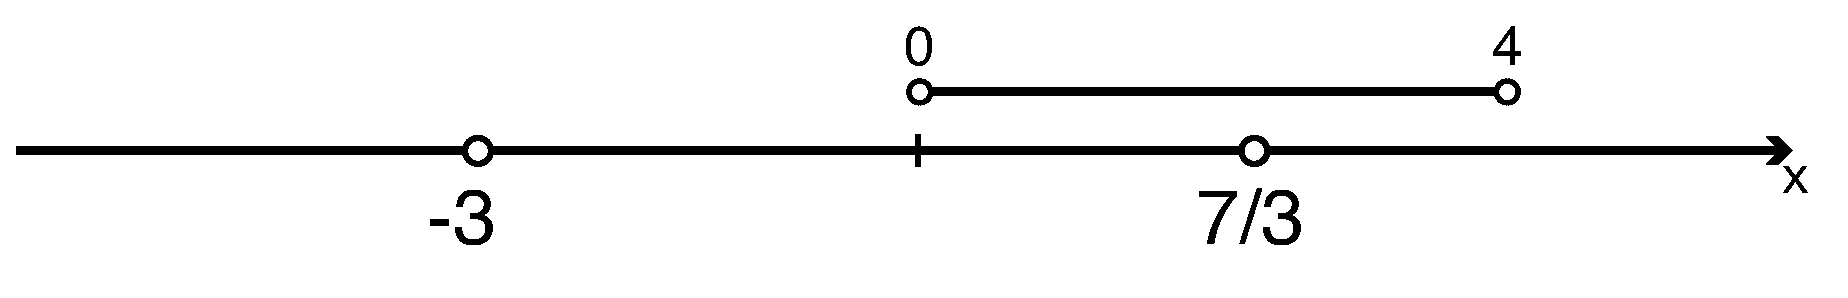
\includegraphics[width=0.70\textwidth]{latex/images/b1p1-026-fig01}
    \end{figure}
    \par Then the graphs of $ A \cap B $, $ A \cup B $, $ A-B $ and $ B-A $
% =======================================================
\end{document}  
